\documentclass[sigconf,nonacm]{acmart}

\begin{document}

\begin{figure*}
    \centering
    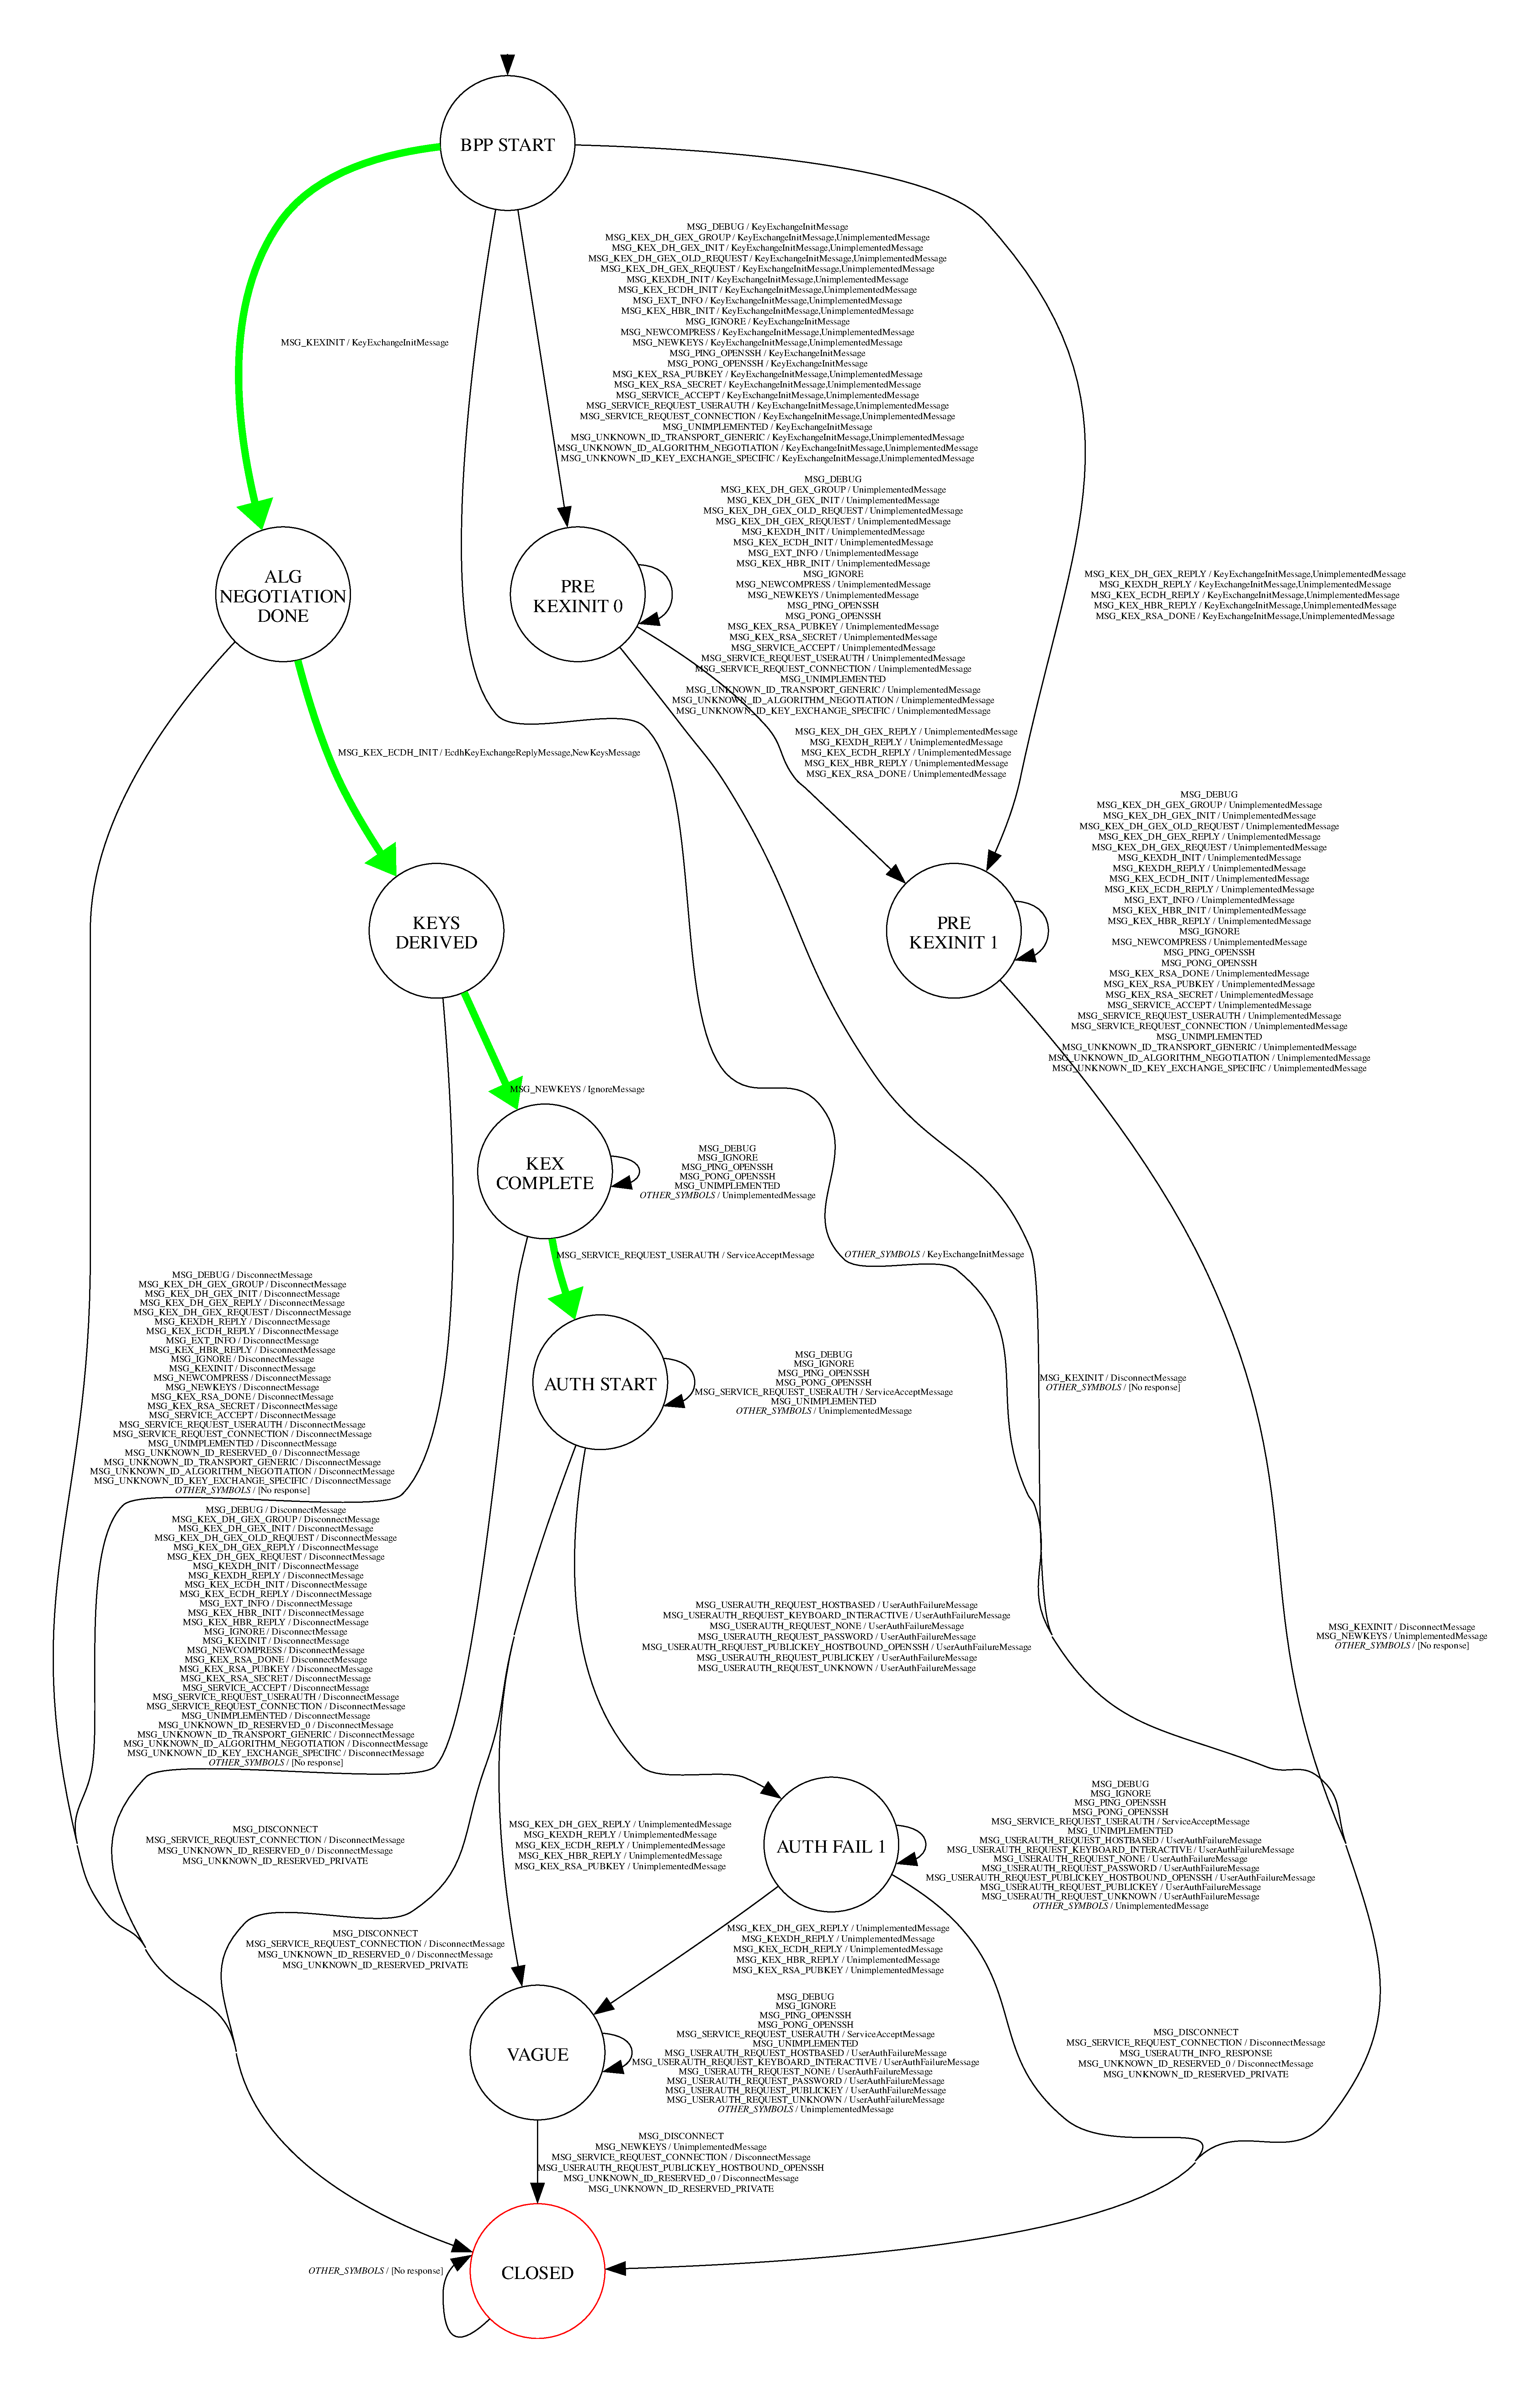
\includegraphics[height=.92\textheight]{img/openssh_9.9p2_ecdh_condensed.pdf}
    \caption*{A condensed representation of the state machine extracted by our state learner from an OpenSSH 9.9p2 server with strict kex enabled. The ``vague'' state is a result of our focus on the transport layer rather than the authentication protocol during the search for counterexamples and may not accurately depict the behavior of the server at that stage.}
    \Description{The figure depicts a complex SSH state machine consisting of ten states and various edges. The happy flow is shown with green arrows. For all edges, there are labels describing the input and output symbols of the Mealy machine for that state transition.}
\end{figure*}

\end{document}
\endinput
